%!TEX root = ../../dissertation.tex
%%%%%%%%%%%%%%%%%%%%%%%%%%%%%%%%%%%%%%%%%%%%%%%%%%%%%%%%%%%%%%%%%%%%%%%%%%%%%%%%
\section{Mobile Reliable Streaming Simulations}
\label{c6:sec:mobilestreamingtestbed}

However, some experiments can not be easily conducted in active measurement testbeds, for example due to the necessary scale to achieve meaningful results. Especially, new protocols or adaptations to existing ones are preferentially first tested in a network simulation. Simulation frameworks are especially important for mobile networks, as acquiring packet-level traces and information about every node in an actual commercially operating cellular network is nigh impossible due to the users' privacy and the provider's business concerns.

While there are some active measurement studies specifically targeted at reliable streaming in mobile networks, e.g., \cite{Muller:2012:EDA:2151677.2151686}, most are conducted either in fixed networks or using simulation frameworks. Therefore, to better evaluate reliable streaming, it would be very desirable to find an existing framework, that covers all important aspect in 3G or 4G mobile networks.

There are a number of network simulators readily available for use, both commercial as well as \gls{FOSS}. But only a small subset of them has the capability (or can be extended) to simulate \gls{3G} or LTE networks. Even further, most radio network capable simulators only concern themselves with the physical radio link and completely neglect all other network paths, especially the core and all control plane signaling interactions. 

The following list overviews current publicly available simulation frameworks with \gls{3G}/\gls{LTE} support:

\begin{itemize}
	\item An external \gls{UMTS} module\footnote{\url{http://net.infocom.uniroma1.it/reti_files/reti_downloads.htm}} is available for the no longer maintained \textbf{ns-2} simulation framework. A further separate collection of patches\footnote{\url{http://seacorn.cs.ucy.ac.cy/eumtssim/}} also extends ns-2 with \gls{UMTS} radio link capabilities~\cite{vranjevs2011use} but it is not publicly available.

	Both are as of August 2014 no longer being developed and not up-to-date to the newest specifications. They also focus solely on the user plane radio physical and link layer of \gls{UMTS}.

	\item Another third-party radio link layer simulation model is available for \textbf{MATLAB}\footnote{\url{http://www.nt.tuwien.ac.at/research/mobile-communications/lte-simulators/}}~\cite{mehlfuhrer2011vienna}.

	\item A standalone \gls{LTE} simulation\footnote{\url{http://telematics.poliba.it/index.php/en/lte-sim}}~\cite{5634134} includes models for some \gls{LTE} nodes, including the \gls{eNB} and \gls{MME} and implements a selection of protocols (\gls{PDCP}, \gls{RLC}, and \gls{RRC}).

	However, the implementation of these nodes and protocols is rudimentary at best and is not even close to the actual specification. Additionally, the simulator lacks a \gls{TCP}/\gls{IP} stack as \gls{IP} is reduced to its basic functionality and \gls{TCP} is completely absent.

	\item A framework dubbed SimuLTE\footnote{\url{https://github.com/inet-framework/simulte}} is available for \textbf{Omnet++}\footnote{\url{http://www.omnetpp.org/}}. Included are the user plane aspects of the radio link and some basic \gls{SGW} and \gls{PGW} functionality.

	\item The \textbf{ns-3}\footnote{\url{http://www.nsnam.org}} simulator already contains an \gls{LTE}/\gls{EPC} module called LENA\footnote{\url{http://networks.cttc.es/mobile-networks/software-tools/lena/}}~\cite{Baldo:2013:OSM:2507924.2507940} with features similar to SimuLTE. Again, only user plane \gls{SGW}/\gls{PGW} functionality is present with an initial \gls{GTP-U} implementation.
\end{itemize}

The goal here is to simulate reliable streaming in a realistic mobile environment. That includes both a complete horizontal network path --- both the radio link as well as the core network --- as well as a vertical network stack --- comprising both user plane and control plane.

Unfortunately, none of the above feature a complete representation, which can be at least partially attributed to the complexity of the \gls{3GPP} specifications. Nonetheless, the simulators could still provide a viable basis for a mobile streaming framework while keeping the limitations in mind.Between these a decision needs to be made as to the basis of the mobile streaming simulation framework. 

Ultimately, the choice fell on ns-3 with the LENA module. Alongside with SimuLTE it has the most complete \gls{LTE} representation. And targeting \gls{LTE} networks seems to be the more future-proof path in the the long term. With the exception of Omnet++, which has comparable capabilities, ns-3's \gls{TCP}/\gls{IP} is much more complete and realistic than that of the other frameworks. Additionally, it can also incorporate the actual \gls{TCP}/\gls{IP} of older Linux kernels with NSC\footnote{\url{http://research.wand.net.nz/software/nsc.php}}. As an additional feature, ns-3 can also act as a network emulator for real network traffic. This will be exploited in the upcoming model.

In the long run, to better represent actual mobile networks the base radio framework in ns-3 would need to be extended with more control plane aspects and adapted to the latest \gls{3GPP} specifications


%%%%%%%%%%%%%%%%%%%%%%%%%%%%%%%%%%%%%%%%%%%%%%%%%%%%%%%%%%%%%%%%%%%%%%%%%%%%%%%%
\subsection{Simulating Mobile Reliable Streaming in ns-3}

With ns-3 chosen and the core network model set, the task is now to define and simulate reliable streaming on top of the \gls{LTE} network. To properly evaluate the setup a number of measurement series also has to be defined and conducted.

Through this simulation testbed, arbitrary reliable streaming playback models can now be tested and optimized for the various conditions and pitfalls of mobile networks. Of special interest could be the relation to mobility phenomenons and issues occurring during handover.

%%
\subsubsection{Simulation and Emulation Setups}

To simplify things, the model behind the progressive streaming measurement framework based on the playback buffer employed in Section~\ref{c3:sec:measurements} can be reused in the simulator.

\begin{figure}[htb]
\centering
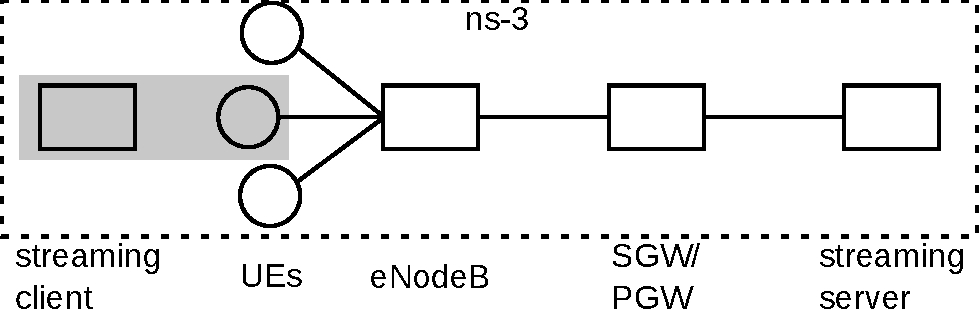
\includegraphics[width=0.6\textwidth]{images/streaming-simulation.pdf}
\caption{\gls{LTE} reliable streaming simulation testbed.}
\label{c5:fig:streaming-simulation}
\end{figure}


The rest of the network model is kept as simple as possible as is visible in Figure~\ref{c5:fig:streaming-simulation}. LENA readily provides implementations for the \glspl{UE}, \gls{eNB}, and a combined \gls{SGW}/\gls{PGW} node. For the streaming simulation two things were added into this network. 

A node which acts as the storage server for the video segments was connected to the Internet-facing link of the \gls{PGW}. The storage server is kept as simple as possible. Upon receipt of a request for a specific segment over \gls{TCP} a dummy segment with the correct size is immediately sent to the client, reusing the open \gls{TCP} connection. \todo{Segments typically have a size of ...?}

The client's playback buffering model is implemented as an application running on the \gls{UE}. The device also initiates the streaming and takes care of requesting each individual segment. However, the segments do not contain actual video data. Rather, the playback simulator just reads the list of frames and their size and synchronizes this information with the received amount of data to correctly calculate the buffer level.

During transmission, the \gls{LTE} framework sets up the lower layer protocols, which includes the radio stack and the \gls{gtp} core network bearer, accordingly. In the simplest model, only one \gls{eNB} and one \gls{UE} are present, to avoid interference with other devices. Moreover, a stationary mobility model with close distance to the transceiver is chosen. The model can be easily extended to factor in multiple devices and a mobility model with handover, all the capabilities are already present in ns-3. However, the simple setup was chosen to measure the upper limit of achievable performance. All of the other factors will undoubtedly reduce th performance. Otherwise, the \gls{LTE} nodes are left at their default configuration, which should yield an overall cell net bandwidth of \SI{80}{\mega\bit\per\second}


%% emu

\begin{figure}[htb]
\centering
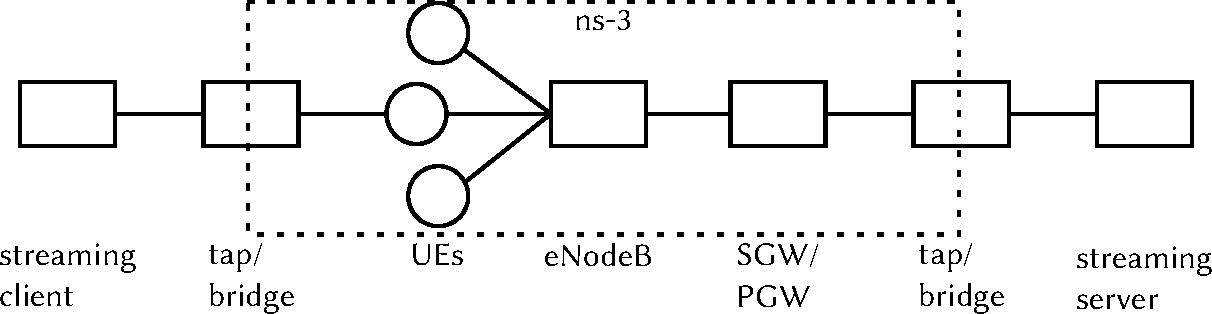
\includegraphics[width=\textwidth]{images/streaming-hybrid.pdf}
\caption{Future testbed iteration: hybrid of ns-3 LTE simulation and actual or emulated streaming client and server bridged to it.}
\label{c5:fig:streaming-hybrid}
\end{figure}

Beyond its application as a pure simulation, a simulated ns-3 \gls{LTE} network could additionally be facilitated as a network emulator. Figure~\ref{c5:fig:streaming-hybrid} demonstrates such a setup. To be able to use it for a streaming emulation in the style of the measurements conducted in Section~\ref{c3:sec:measurements} a bridging device would need to be added on each side of the network, that interfaces with a real testbed network. The only effect of the simulated part is then to alter the \gls{QoS} parameters of the link according to its model. This approach is ideally suited to quickly test existing and already implemented streaming solutions for use with a mobile network and saves the effort of reimplementing them as a simulation model.


%%
\subsubsection{Simulated Streaming Model}
Reliable streaming type implemented:

According to the classification and playback modeling from Sections~\ref{c3:sec:background} and \ref{c3:sec:model} the simulated model is a pull-based segmented video streaming system using \gls{TCP}. Two streaming models are suggested here, with the first suited for plain reliable streaming and the second modified to utilize the benefits of adaptive streaming.


%%
\paragraph{Four Threshold Segmented Streaming Model}

4 threshold segmented streaming
	Playback stop if below threshold 1 default \SI{0.5}{\second} buffered time can also be simply 0 (or no complete frame in the buffer)
	Transmission start if below threshold 2 (request new segments), default \SI{2.5}{\second}
	Playback start if above threshold 3, default \SI{5}{\second}
	Transmission stop if above threshold 4 (request no new segments)

to avoid behavior similar to stop-and-go transport protocols, new segments need to be requested ahead of time, so that the full bandwidth is always utilized. This becomes more critical the higher the overall latency is, as the gaps would become larger there if not requested in time.

Depending on the relation of transmission bandwidth to playback bitrate
in optimal conditions, a player with this strategy should always bounce between thresholds 2 and 4 and never stop playing intermittently.


directly on top of TCP
pull-based with request per segment; could also use HTTP here, but should not make much difference, only slightly more overhead through http header


\begin{figure}[htb]
\centering
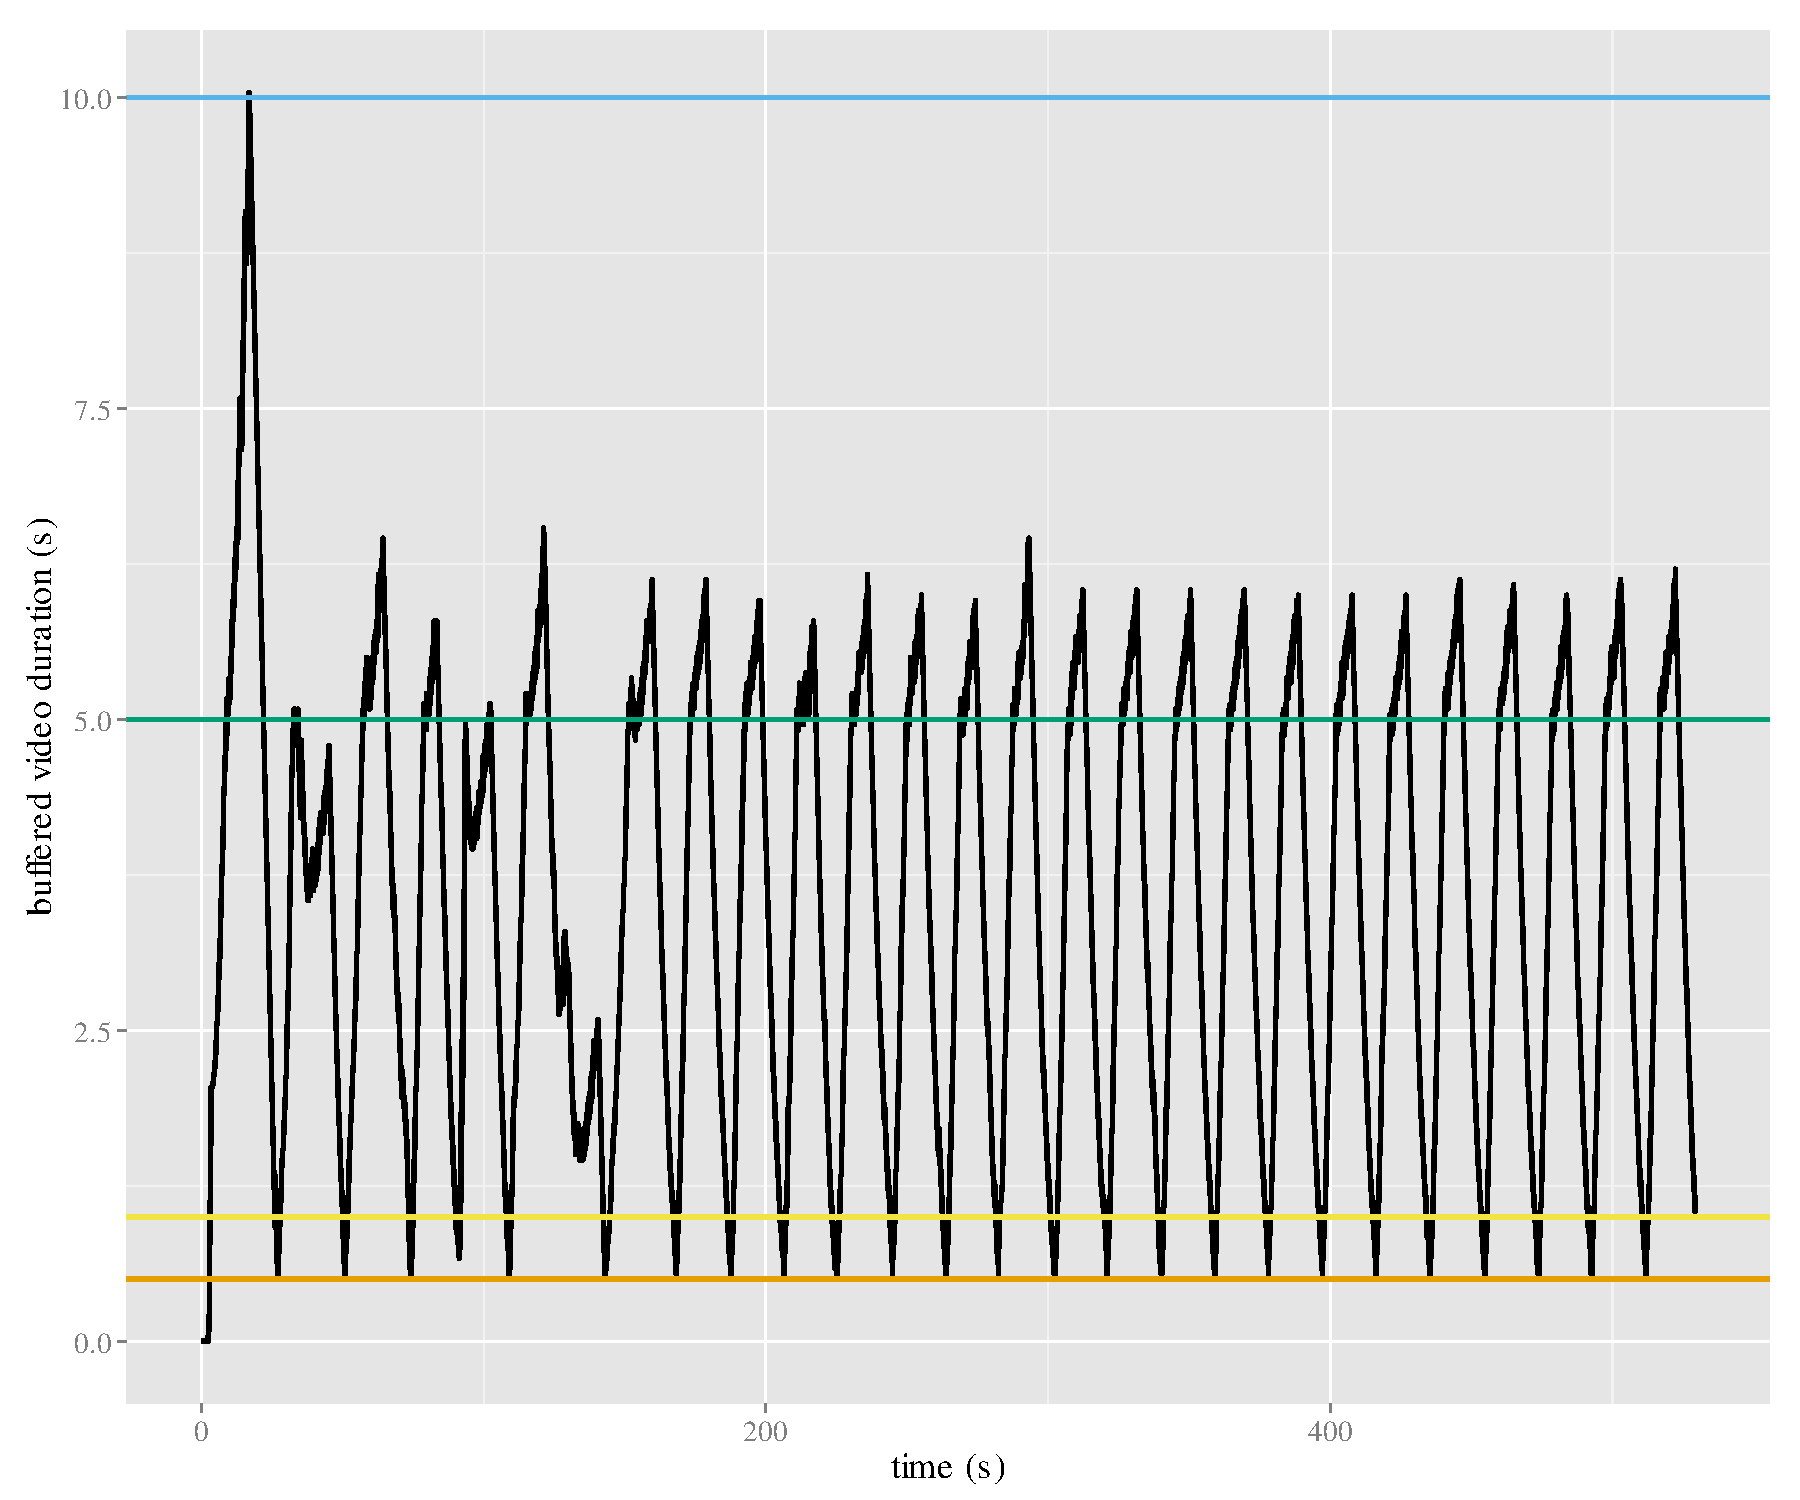
\includegraphics[width=1.0\textwidth]{images/R-ltesim-plotbuffer-time.pdf}
\caption{R-ltesim-plotbuffer-time.pdf}
\label{c5:fig:ltesim-plotbuffer-time}
\end{figure}


%%
\paragraph{Six Threshold Window Scaling Adaptive Streaming Model}

planned not fully implemented 
6 threshold adaptive reliable streaming


lower segment quality by 1 threshold 5
increase segment quality by 1 threshold 6
	if T6 is hit again, or buffer is still increasing, then also keep increasing the segment quality
	need to always keep track of video bitrate and transmission speed in current window for this to work properly!
	recheck conditions every x seconds and dont change quality to rapidly as this might cause irritation

	Same goes for T5 in the other direction

	T6 should be between T3 and T4
	T5 should be between T1 and T2

%% ! <-- !
%%



%%
\subsubsection{Scenario Evaluation}
Evaluated Scenarios (and scenarios that are worthy of evaluation in the fture)

 test case 1: adaptability of diverse reliable video streaming to LTE and mobile networks, by altering latency, loss, bandwidth

 test case 2a (future): influence of mobility effects on reliable streaming
 test case 2b (future): effect of cross-layer information in mobility case



test videos:

video 1:
MP4 container
\SI{318}{\second} duration
\SI{20.2}{\mebi\byte}
H.263 video 352x288
29.97 fps
\SI{504}{\kilo\bit\per\second} video bitrate
((we dont emulate audio, dont we?)
AAC audio, 11KHz
\SI{24.0}{\kilo\bit\per\second} audio bitrate)

\SI{531.0}{\kilo\bit\per\second} overall bitrate

video 2:
AVI container
\SI{596}{\second}
MPEG-4 Simple Profile, 1920x1080
24.00 fps
\SI{12}{\mega\bit\per\second} video bitrate
AC-3 audio, 48Khz
\SI{448}{\kilo\bit\per\second} audio bitrate

\SI{12.5}{\mega\bit\per\second} overall bitrate

video 3:
DivX container
\SI{602}{\second}
MPEG-4 (nicht AVC), 720x400
29.97 fps
\SI{3596}{\kilo\bit\per\second} video bitrate
MP3 audio, 44.1Khz
\SI{128}{\kilo\bit\per\second} audio bitrate

\SI{3735}{\kilo\bit\per\second} overall bitrate


%%
Series 1: Limited bandwidth on the fixed network path



\begin{figure}[htb]
\centering
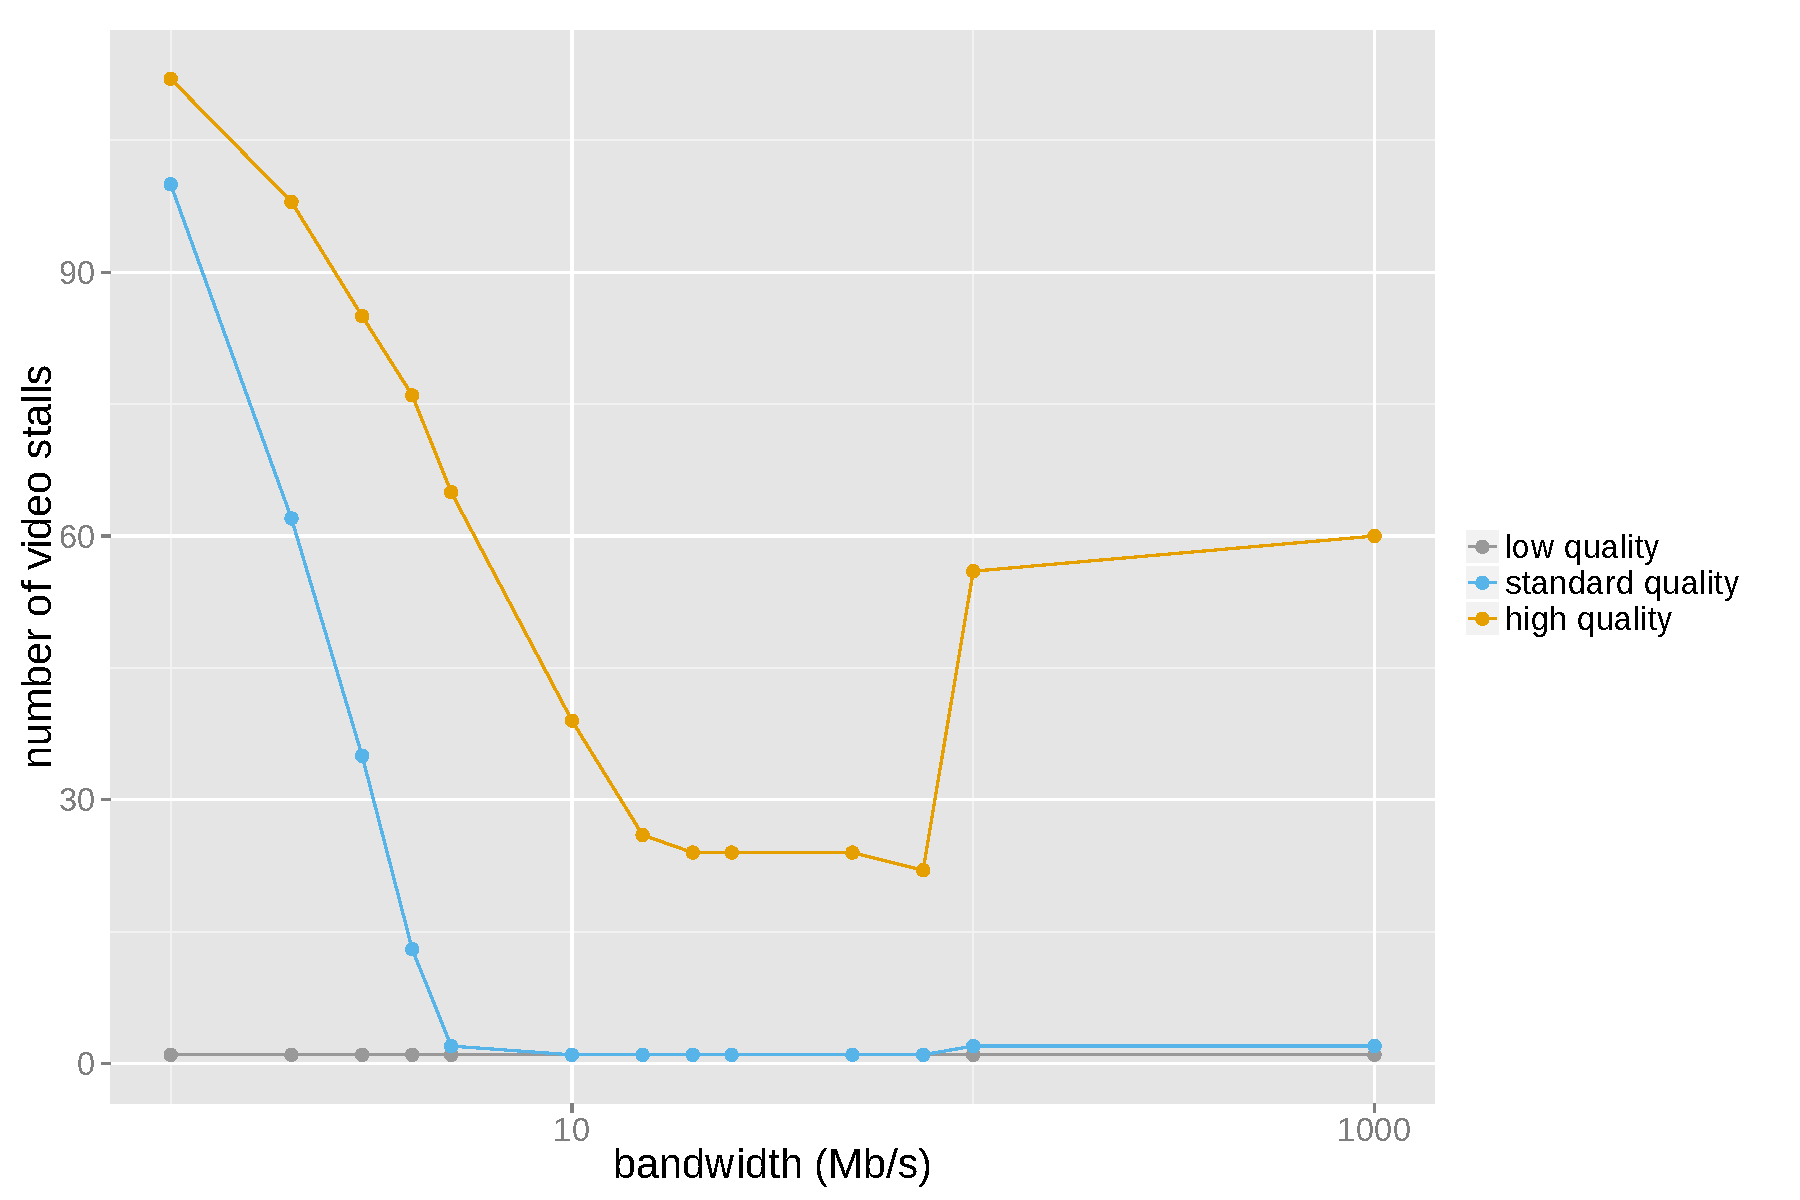
\includegraphics[width=1.0\textwidth]{images/R-ltesim-bwseries-numstalls.pdf}
\caption{R-ltesim-bwseries-numstalls.pdf}
\label{c5:fig:ltesim-bwseries-numstalls}
\end{figure}

\begin{figure}[htb]
\centering
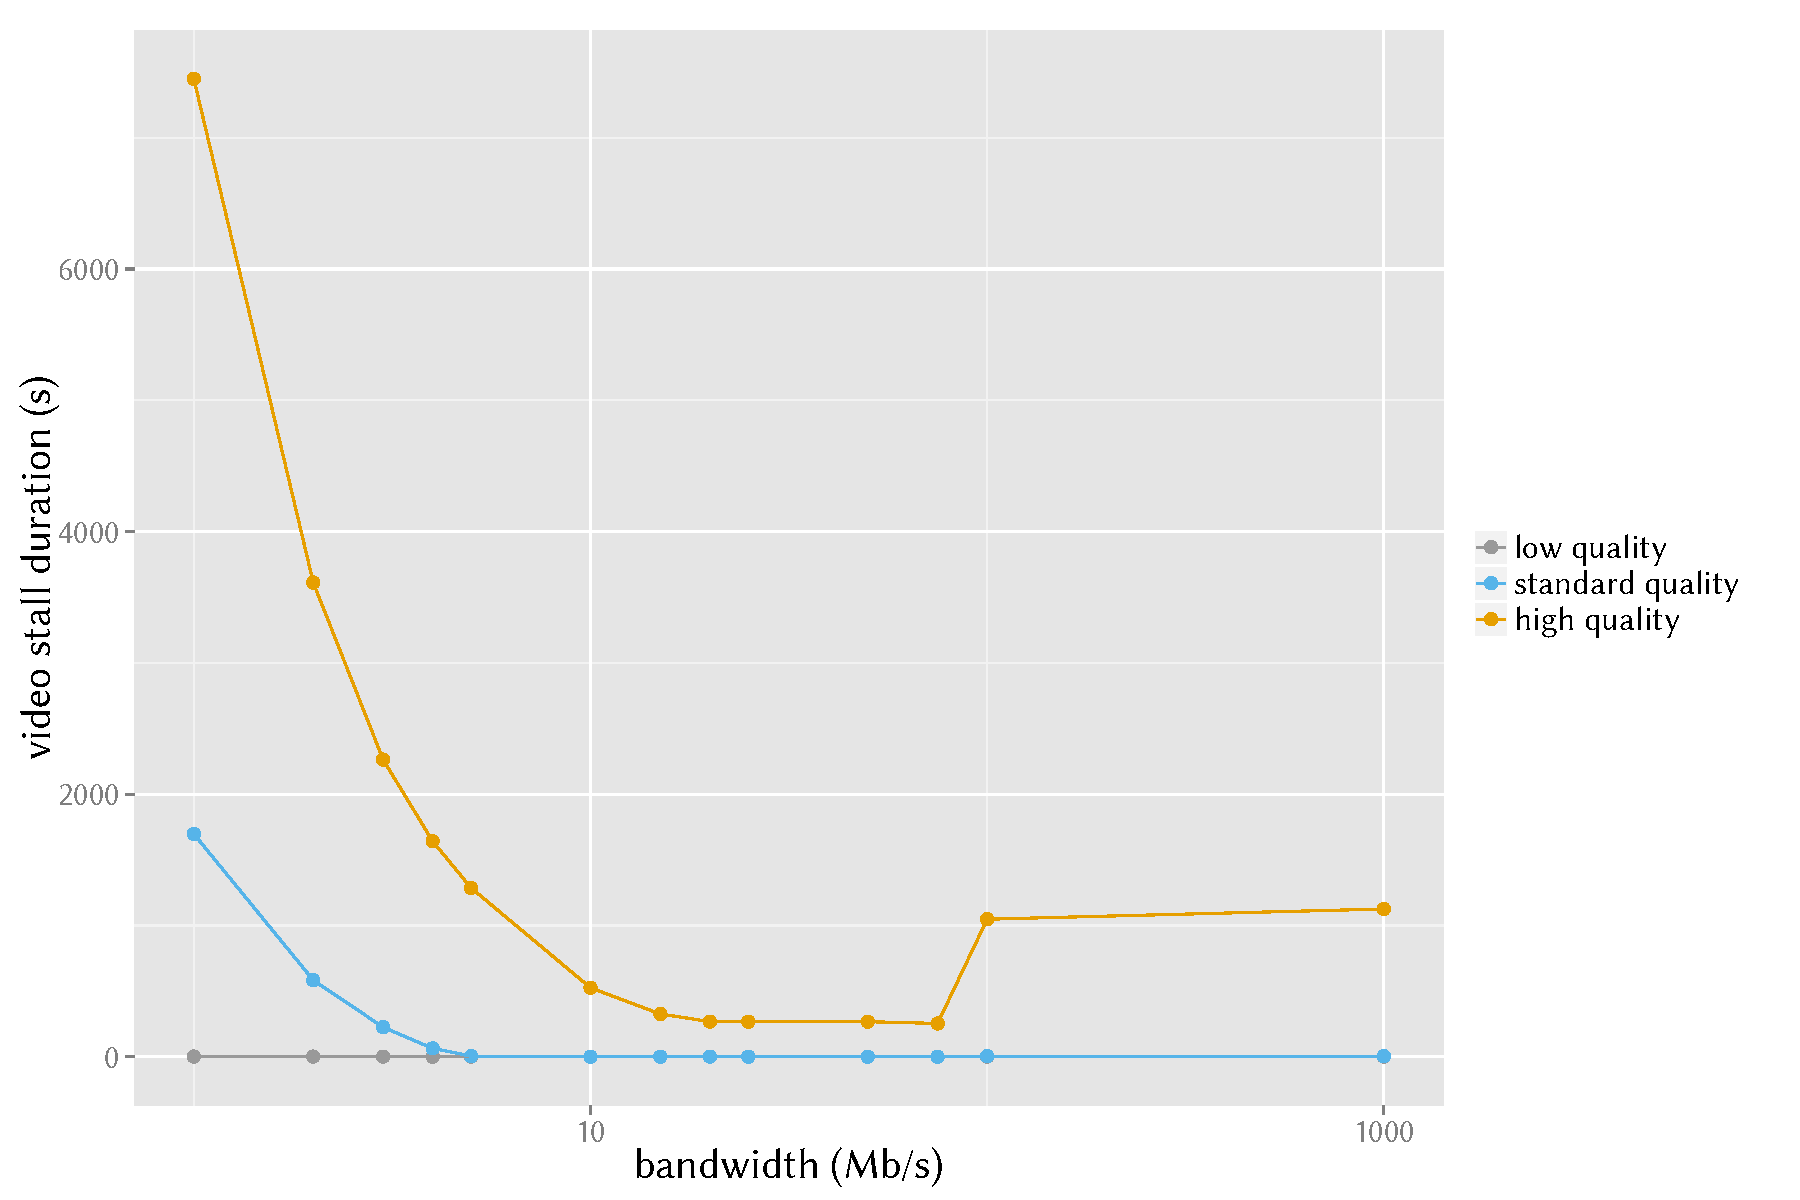
\includegraphics[width=1.0\textwidth]{images/R-ltesim-bwseries-stallduration.pdf}
\caption{R-ltesim-bwseries-stallduration.pdf}
\label{c5:fig:ltesim-bwseries-stallduration}
\end{figure}


%%
Series 2: Deterministically increased latency on the fixed network path

\begin{figure}[htb]
\centering
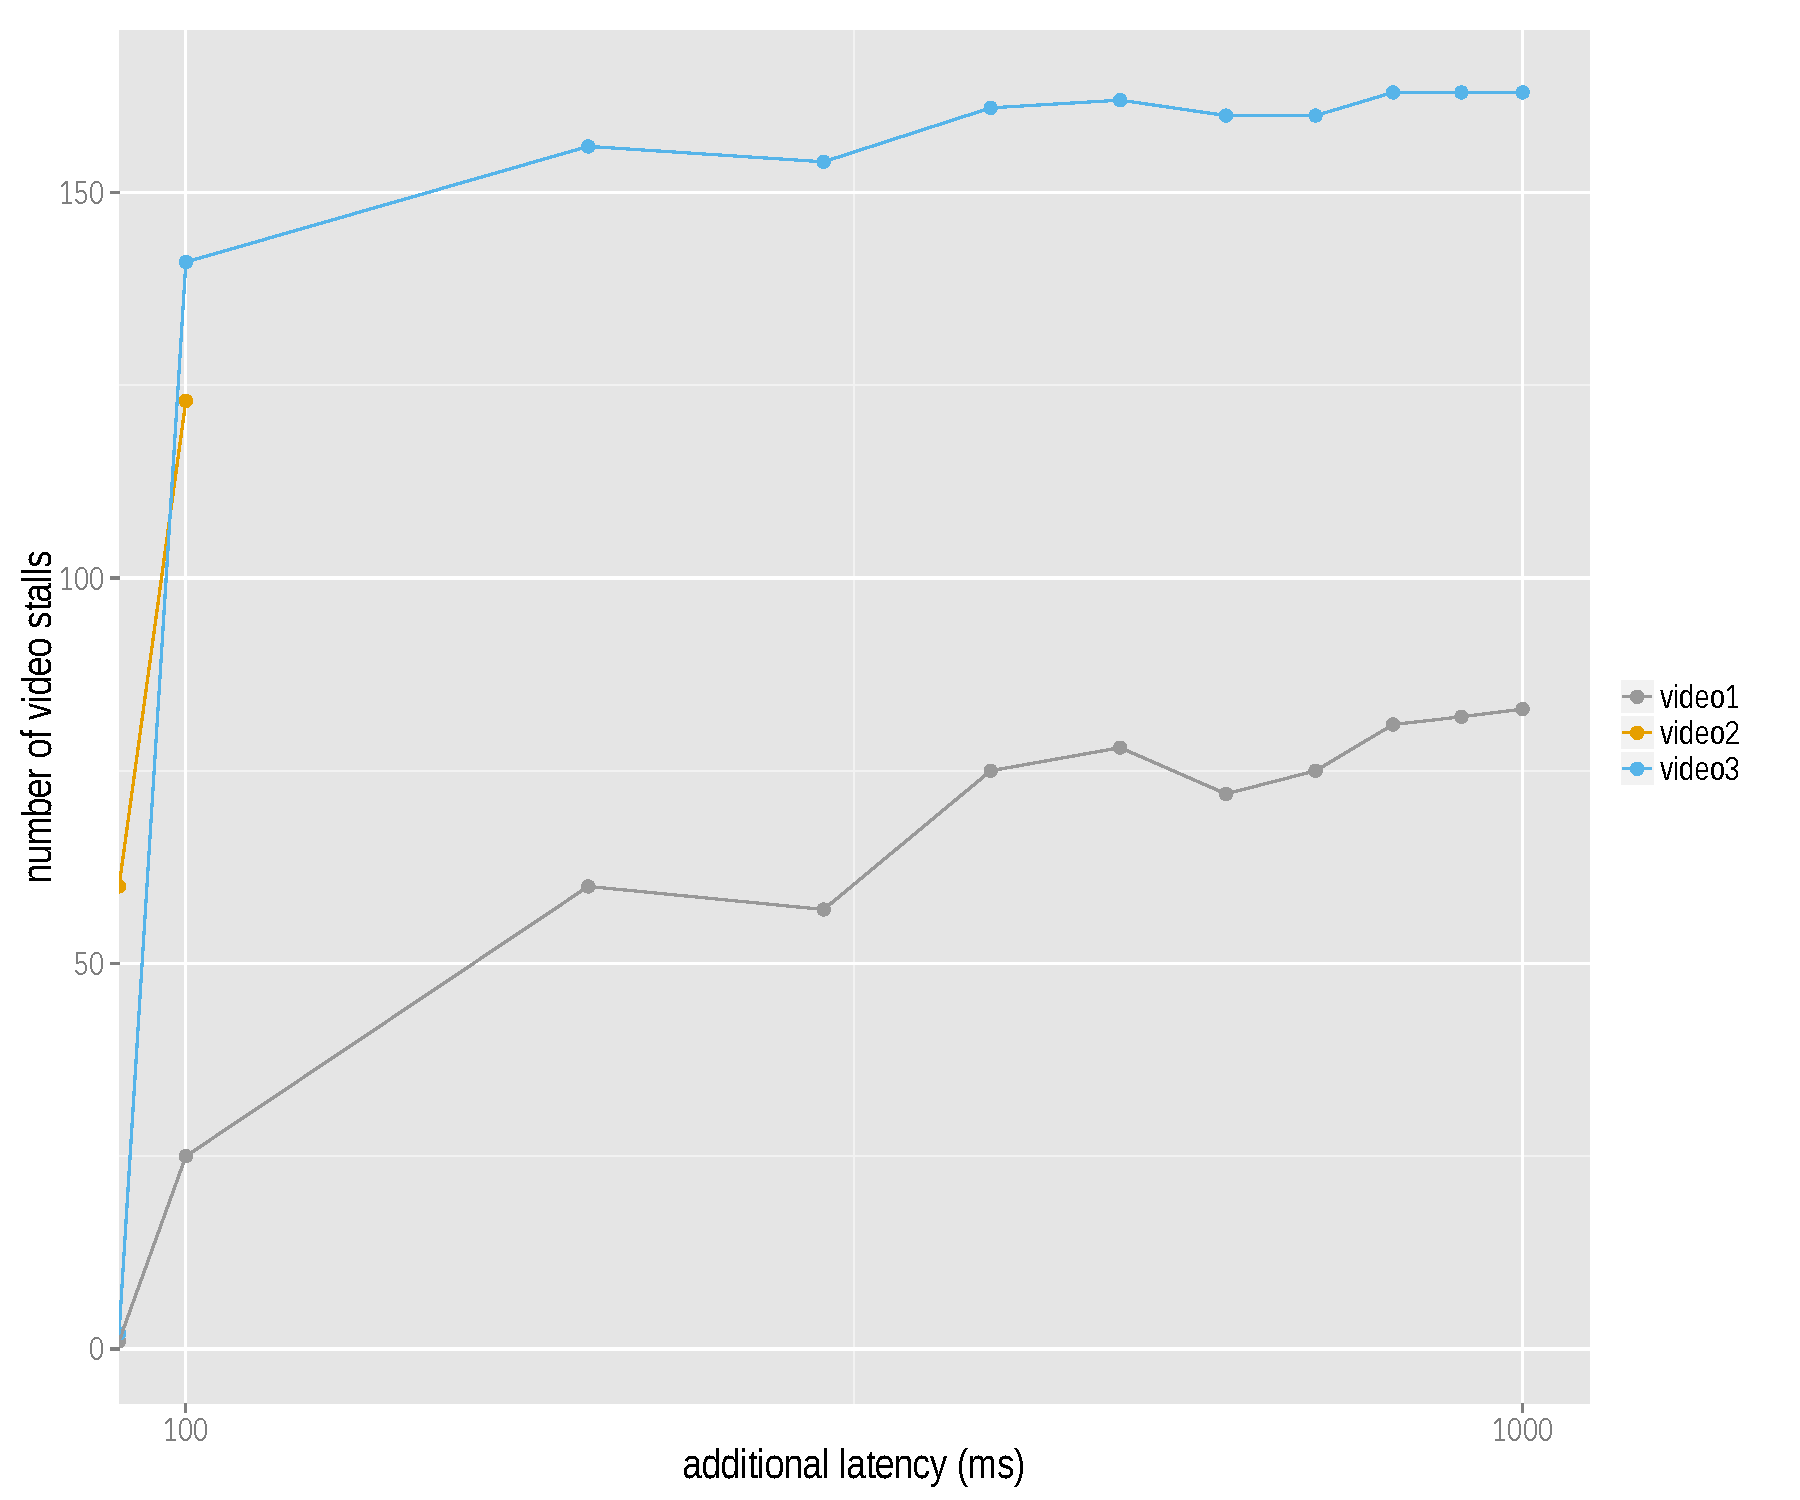
\includegraphics[width=1.0\textwidth]{images/R-ltesim-latencyseries-numstalls.pdf}
\caption{R-ltesim-latencyseries-numstalls.pdf}
\label{c5:fig:ltesim-latencyseries-numstalls}
\end{figure}

\begin{figure}[htb]
\centering
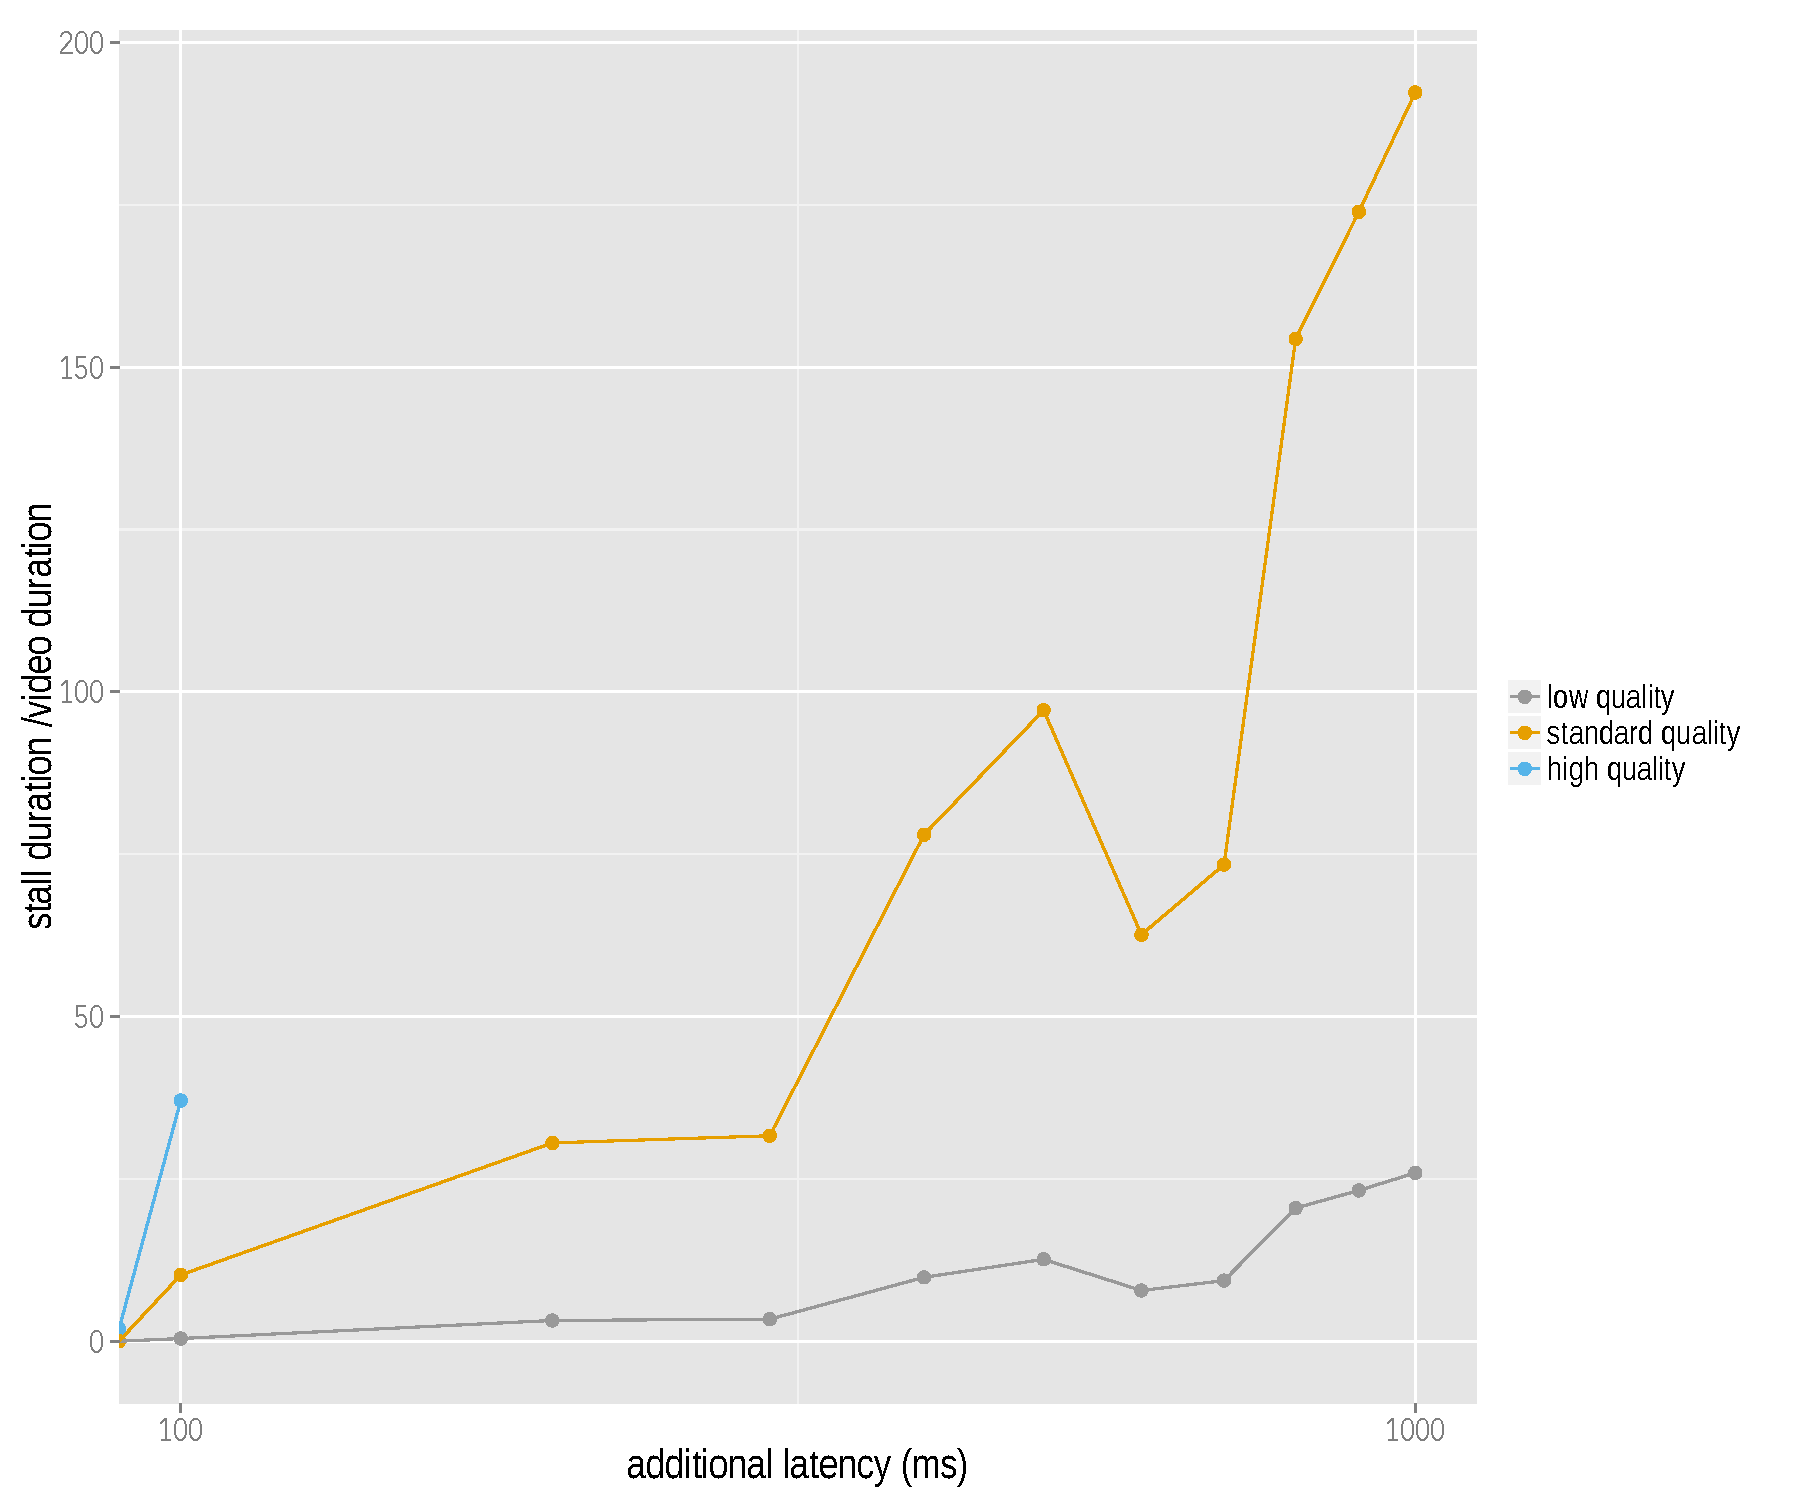
\includegraphics[width=1.0\textwidth]{images/R-ltesim-latencyseries-stallduration.pdf}
\caption{R-ltesim-latencyseries-stallduration.pdf}
\label{c5:fig:ltesim-latencyseries-stallduration}
\end{figure}

%%
Series 4: Packet loss on the fixed network path






% \begin{figure}[htb]
% \centering
% 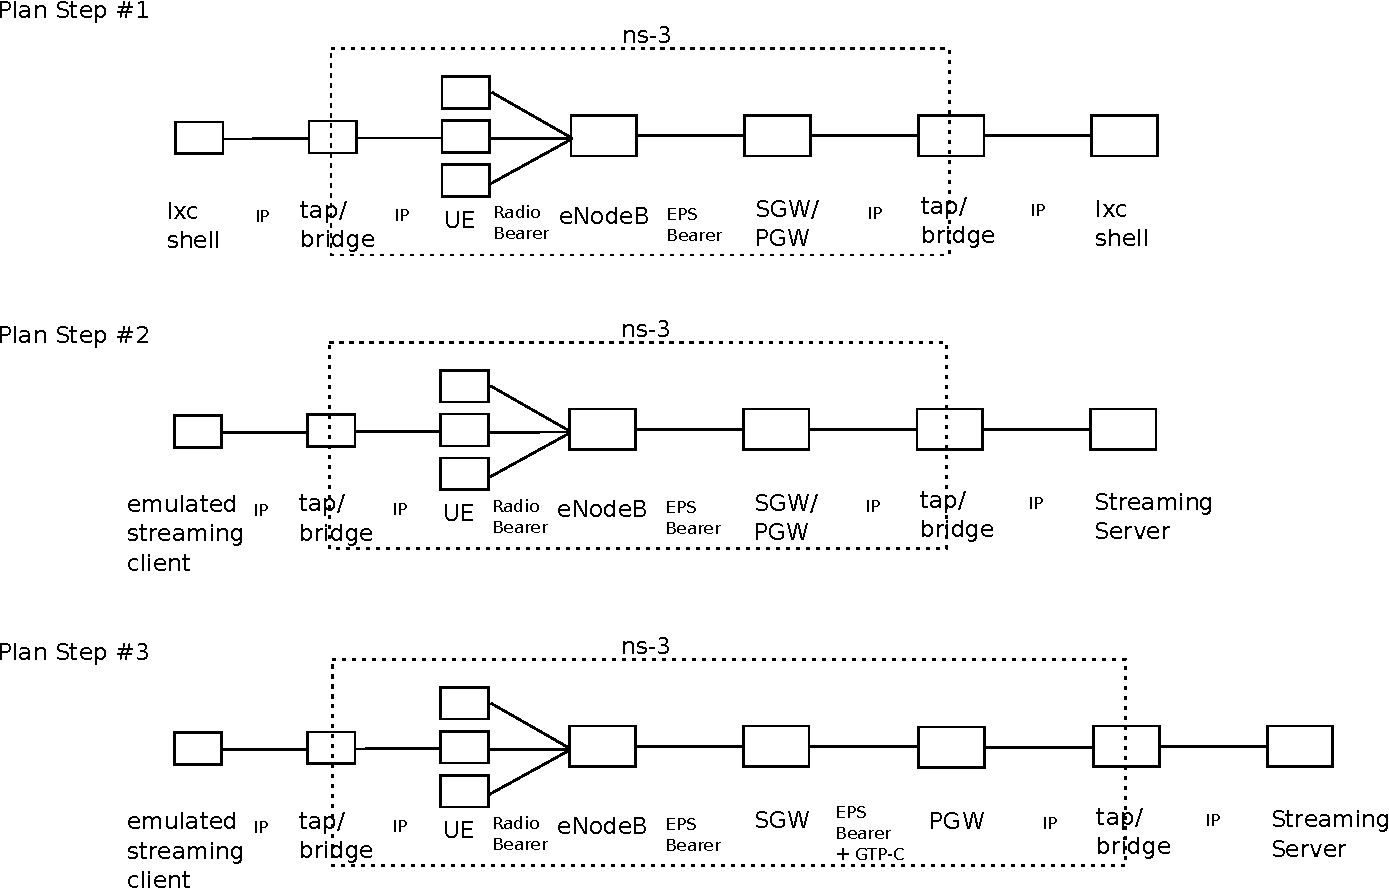
\includegraphics[width=\textwidth]{images/lte-testbed.pdf}
% \caption{\gls{LTE} Streaming Evaluation Setup and Action Plan}
% \label{fig:lte-testbed}
% \end{figure}



% \url{http://www.valid8.com/UMTS_Core_Network_Simulator.html} Not publicly available and commercial
% also seems to focus on the circuit switched domain


% Only commercial: UMTS model in OPNET (which was renamed to Riverbed Modeler)\footnote{\url{http://www.riverbed.com/products/performance-management-control/network-performance-management/network-simulation.html}} 
% again radio and user plane focused

%\url{http://www.nsnam.org/docs/release/3.20/doxygen/group__lte.html}
%\url{http://www.nsnam.org/docs/release/3.20/models/html/lte.html}

%Reasoning why ns-3/LENA will be used here.
%but combined with ns-3 offers almost complete representation of a vanilla network and transport level network stack


%performance: eNB has 25 resource block each up/down; suggests 5Mhz BW
%https://groups.google.com/forum/#!searchin/ns-3-users/lte/ns-3-users/dwMjWwJBdBw/wfWCcRctN4EJ